\chapter{Numerical Characterization of Shear Wave Speed Quantification}
	\label{chap:shear}
	\section{Introduction}
		Shear wave speed quantification offers the most desirable method of detecting early deep tissues injuries as it takes the transducer-generated external deformation force that is the chief benefit of ARFI imaging and combines it with a quantitative measure of tissue elasticity rather than the qualitative measures used in both quasi-static elastography and ARFI imaging. Specifically, monitoring the speed of shear waves that are generated in the tissue as a response to a localized acoustic radiation force allows the calculation of tissue stiffness which may again be used as an analogue of tissue health. Further, since the technique is quantitative in nature, tissue stiffness may be accurately tracked over time, enabling physicians to appropriately monitor the progression and treatment of a given deep tissue injury on a per-patient basis.

	\section{Method}
	\label{sec:shear_method}
		In order to investigate the sensitivity and applicability of shear wave speed quantification for the early detection of deep tissue injuries, a combination of k-space pseudospectral models of acoustic wave propagation and time-domain finite-element models of tissue deformation were employed. The theory and procedure behind both the generalized acoustic simulations using k-space pseudospectral models and time-dependent solid mechanics finite-element models used here were presented in Chapter \ref{chap:arfi}. As an alternative to monitoring the dynamic response of tissue at the focal point as in ARFI imaging, shear wave speed quantification tracks the velocity of shear waves which radiate laterally outward from the focal point of an ARFI load. If the focal point is positioned such that the generated shear waves propagate through a lesionous region and the speed of the generated shear wave is monitored, the stiffness of that region may be calculated.

		\subsection{Shear Wave Speed}
			The foundation of shear wave speed quantification with regards to detecting lesionous regions lies in the quantifiable relationship between shear wave speeds and tissue stiffness. This relationship between shear wave speed and tissue stiffness is derived here, assuming a linear elastic, isotropic material. Soft tissue is generally considered a viscoelastic material and as such modifications to the linear elastic wave speed are taken into account.

			Equation \ref{equ:shear_constitutive} represents the constitutive equation of a linear elastic material where the strain tensor is defined as per equation \ref{equ:shear_strain_tensor} such that equation \ref{equ:shear_constitutive_complete} holds true.

			\begin{equation}
				\label{equ:shear_constitutive}
				\sigma_{ij} = \lambda \delta_{ij} \varepsilon_{kk} + 2 \mu \varepsilon_{ij}
			\end{equation}

			\begin{equation}
				\label{equ:shear_strain_tensor}
				\varepsilon_{ij} = \frac{1}{2}\left(u_{i,j} + u_{j,i}\right)
			\end{equation}

			\begin{equation}
				\label{equ:shear_constitutive_complete}
				\sigma_{ij} = \lambda \varepsilon_{ii} \delta_{ij} + \mu \left(u_{i,j} + u_{j,i}\right)
			\end{equation}

			Neglecting time-invariant body loads, the balance of linear momentum is given for a linear elastic continuum is given in equation \ref{equ:shear_balance_momentum}.

			\begin{equation}
				\label{equ:shear_balance_momentum}
				\sigma_{ij,j} = \rho \ddot{u_i}
			\end{equation}

			Substituting equation \ref{equ:shear_constitutive_complete} into equation \ref{equ:shear_balance_momentum} yields equation \ref{equ:shear_momentum_constitutive} which may be rearranged into equation \ref{equ:shear_momentum_constitutive_rearranged} by noting that $\varepsilon_{ii,j} = u_{j,ij}$.

			\begin{equation}
				\label{equ:shear_momentum_constitutive}
				\lambda \varepsilon_{ii,j} + \mu\left(u_{i,jj} + u_{j,ij}\right) = \rho \ddot{u_i}
			\end{equation}

			\begin{equation}
				\label{equ:shear_momentum_constitutive_rearranged}
				\rho \ddot{u_i} = \left(\lambda + \mu\right)u_{j,ji} + \mu u_{i,jj}
			\end{equation}

			Utilizing the Helmholtz decomposition of the particle displacement given in equation \ref{equ:shear_helmholtz_decomp}, equation \ref{equ:shear_momentum_constitutive_rearranged} becomes equation \ref{equ:shear_helmholtz_subbed}.

			\begin{equation}
				\label{equ:shear_helmholtz_decomp}
				u_i = \partial_i \phi + \varepsilon_{ijk}\partial_j\psi_k
			\end{equation}

			\begin{equation}
				\label{equ:shear_helmholtz_subbed}
				\nabla\left[\left(\lambda + 2\mu\right) \nabla^2 \phi - \rho \ddot{\phi}\right] + \nabla \times \left[\mu \nabla^2 \vec{\psi} - \rho\ddot{\vec{\psi}}\right] = 0
			\end{equation}

			Examining the transverse propagation component of equation \ref{equ:shear_helmholtz_subbed} in one direction yields the familiar shear wave equation given in equation \ref{equ:shear_wave_equation} such that the shear wave speed is given by equation \ref{equ:shear_wave_speed}.

			\begin{equation}
				\label{equ:shear_wave_equation}
				0 = \frac{\partial^2 \vec{\psi}}{\partial x^2} - \frac{\rho}{\mu}\frac{\partial^2 \vec{\psi}}{dt^2}
			\end{equation}

			\begin{equation}
				\label{equ:shear_wave_speed}
				c_T = \sqrt{\frac{\mu}{\rho}}
			\end{equation}

			While the above equation holds for linear elastic materials, soft tissues in the human body are generally considered viscoelastic \note[KH]{Add citation}. In the case of viscoelastic tissues, complex Lam\'{e} parameters must be used, such that the shear wave speed is represented by equation \ref{equ:shear_wave_speed_complex} \note[KH]{Add citation}. Note that viscoelastic shear wave speeds of viscoelastic tissues are generally acquired through empirical measurements rather than any sort of mathematical derivation \note[KH]{Add citation}.

			\begin{equation}
				\label{equ:shear_wave_speed_complex}
				c_T = \sqrt{\frac{\mu^*}{\rho}}
			\end{equation}

		\subsection{Model Set Up}
		\label{subsec:model_setup}
			In order to study the feasibility of using shear wave speed quantification to detect and monitor deep tissue injuries, a collection of deep tissue injury models were investigated including: spherical lesions with hard and soft boundaries, clusters of small lesions that make up a larger lesionous region, and a lesion with mri-acquired geometry \cite{solis13} embedded in geometry obtained from a Visible Human slice \cite{visiblehuman}. Each model investigated numerous parameters relating to the detection of lesions including ARFI focal depth, ARFI interrogation frequency, lesion size, distance of the focal point from the lesion (lesion offset), lesion blur radius, clustered lesion density, the size of individual lesions in the clustered lesion model, and the size and altitude of the lesion in the Visible Human model. The range of parameters investigated for each model are summarized in Table \ref{tab:shear-parametervalues}.

			Figs. \ref{fig:shear_schematics} portray the schematics of the lesion models investigated. Note that shear wave speed quantification typically applies the acoustic radiation force impulse to a location of tissue adjacent to the desired region such that the shear waves are fully developed by the time they reach the investigated region.

			\begin{figure*}[!htb]
				\centering
				\subfloat[]{
					\begin{tikzpicture}[x=0.045\textwidth, y=0.045\textwidth, draw=black, text=black, fill=black]
						% the main domain area
						\draw[fill=tissueColour] (0, 0) rectangle(10, 10);

						% the lesion
						\draw[fill=lesionColour] (7, 6) circle(0.5);

						% the lesion center marks
						\draw (6.4, 6) -- (6.9, 6);
						\draw (7.1, 6) -- (7.6, 6);
						\draw (6.95, 6) -- (7.05, 6);
						\draw (7, 5.4) -- (7, 5.9);
						\draw (7, 6.1) -- (7, 6.6);
						\draw (7, 5.95) -- (7, 6.05);

						% the lesion radius
						\draw[<-] (7.3536, 5.6464) -- (8, 5);
						\draw (7.85, 5) node[right]{\scriptsize $\diameter S$};

						% the lesion depth
						\draw (6, 6) -- (6.5, 6);
						\draw[<-] (6.25, 10) -- (6.25, 8.25);
						\draw (6.25, 8) node{\scriptsize $d$};
						\draw[->] (6.25, 7.75) -- (6.25, 6);

						% the lesion offset
						\draw (7, 5.5) -- (7, 5);
						\draw[<-] (5, 5.25) -- (5.5, 5.25);
						\draw[->] (6.5, 5.25) -- (7, 5.25);
						\draw (6, 5.25) node{\scriptsize $d_{off}$};

						% the centerline
						%\draw (5, -0.1) -- (5, 4.5);
						%\draw (5, 4.6) -- (5, 5.4);
						%\draw (5, 5.5) -- (5, 10.1);
						\draw (5, 0) -- (5, 1.9);
						\draw (5, 1.95) -- (5, 2.05);
						\draw (5, 2.1) -- (5, 3.9);
						\draw (5, 3.95) -- (5, 4.05);
						\draw (5, 4.1) -- (5, 5.9);
						\draw (5, 5.95) -- (5, 6.05);
						\draw (5, 6.1) -- (5, 7.9);
						\draw (5, 7.95) -- (5, 8.05);
						\draw(5, 8.1) -- (5, 10);

						% the domain width
						\draw (0, 10.1) -- (0, 10.5);
						\draw[<-] (0, 10.25) -- (4.25, 10.25);
						\draw (5, 10.25) node{\scriptsize \SI{10}{\cm}};
						\draw[->] (5.75, 10.25) -- (10, 10.25);
						\draw (10, 10.1) -- (10, 10.5);

						% the domain depth
						\draw (10.1, 0) -- (11, 0);
						\draw[<-] (10.75, 0) -- (10.75, 4.75);
						\draw (10.75, 5) node{\scriptsize \SI{10}{\cm}};
						\draw[->] (10.75, 5.25) -- (10.75, 10);
						\draw (10.1, 10) -- (11, 10);

					\end{tikzpicture}
					\label{fig:shear_schematic_single}
				}
				~
				\subfloat[]{
					\begin{tikzpicture}[x=0.045\textwidth, y=0.045\textwidth, draw=black, text=black, fill=black]
						% the main domain area
						\draw[fill=tissueColour] (0, 0) rectangle(10, 10);

						% the lesion
						\draw (7, 6) node{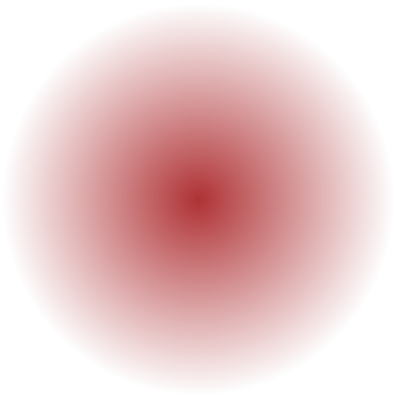
\includegraphics[width=0.045\textwidth]{assets/shear/images/blurredLesion.png}};
						\draw (7, 6) circle(0.5);

						% the lesion radius
						\draw[<-] (7.3536, 5.6464) -- (8, 5);
						\draw (7.85, 5) node[right]{\scriptsize $\diameter S$};

					\end{tikzpicture}
					\label{fig:shear_schematic_blur}
				}
				
				\subfloat[]{
					\begin{tikzpicture}[x=0.045\textwidth, y=0.045\textwidth, draw=black, text=black, fill=black]
						% the main domain area
						\draw[fill=tissueColour] (0, 0) rectangle(10, 10);

						% the lesion
						\draw (7, 6) node{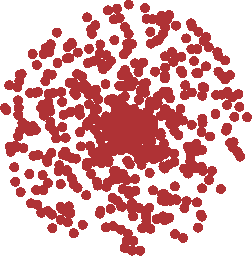
\includegraphics[width=0.045\textwidth]{assets/shear/images/clusteredLesion.png}};
						\draw (7, 6) circle(0.5);

						% the lesion radius
						\draw[<-] (7.3536, 5.6464) -- (8, 5);
						\draw (7.85, 5) node[right]{\scriptsize $\diameter S$};

						% blob size
						\draw[<-] (6.9, 5.9) -- (6, 5) node[left]{\scriptsize $r_{bl}$};

					\end{tikzpicture}
					\label{fig:shear_schematic_clustered}
				}
				~
				\subfloat[]{
					\begin{tikzpicture}[x=0.045\textwidth, y=0.045\textwidth, draw=black, text=black, fill=black]
						% the human stuffz
						\draw (5, 5) node{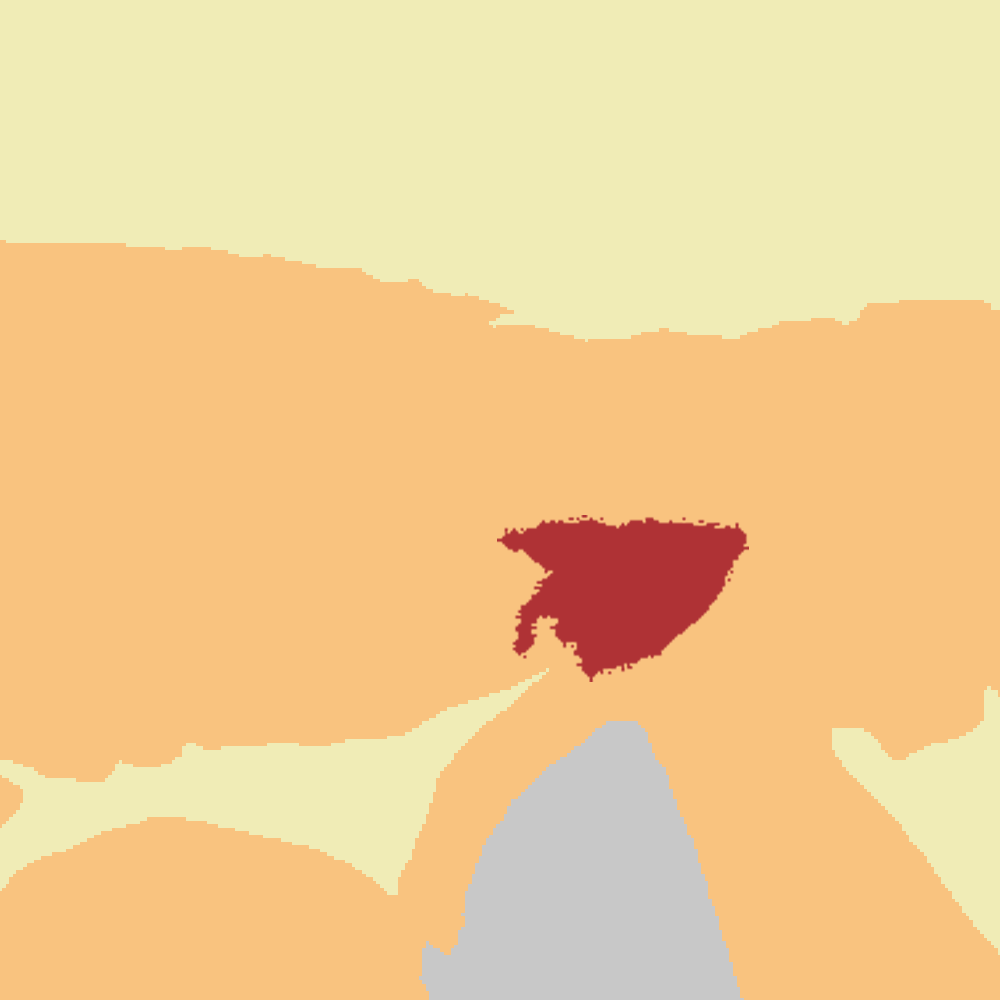
\includegraphics[width=0.45\textwidth]{assets/shear/images/humanSchematic.png}};

						% the main domain area
						\draw (0, 0) rectangle(10, 10);

						% the depth
						\draw (7.25, 4) -- (8, 4);
						\draw (7.75, 7) node{\scriptsize $d$};
						\draw[<-] (7.75, 10) -- (7.75, 7.25);
						\draw[->] (7.75, 6.75) -- (7.75, 4);

						% the size
						\draw (5, 4.7) -- (5, 5.5);
						\draw (7.25, 4.7) -- (7.25, 5.5);
						\draw (6.125, 5.25) node{\scriptsize $\diameter S$};
						\draw[<-] (5, 5.25) -- (5.75, 5.25);
						\draw[->] (6.5, 5.25) -- (7.25, 5.25);

					\end{tikzpicture}
					\label{fig:shear_schematic_human}
				}
				\caption[Schematic of shear wave speed quantification-investigated lesions]{Schematics of the lesion models that were investigated using shear wave speed quantification showing \protect\subref{fig:shear_schematic_single} a spherical hard-boundaried lesion, \protect\subref{fig:shear_schematic_blur} a spherical blurred-boundary lesion, \protect\subref{fig:shear_schematic_clustered} a cluster of numerous small lesions composing a larger lesionous region, and \protect\subref{fig:shear_schematic_human} the geometry from an MRI-acquired deep tissue injury overlaid on a slice from the Visible Human Project such that the injury lesion was located immediately superior to an ischial tuberosity.}	
				\label{fig:shear_schematics}
			\end{figure*}

			\begin{table}[!htb]
				\centering
				\caption[Shear wave speed quantification model investigated parameters]{Range of values of investigated parameters}
				\label{tab:shear-parametervalues}
				\begin{tabular}{lcc}
					\toprule
					Parameter & Symbol & Values \\
					\midrule
					Lesion depth & $d$ & $[1, 2, 3, 4, 5, 6, 7, 8, 9]$\,\si{\cm} \\
					Lesion diameter & $\diameter S$ & $[0.5, 1.0, 2.0, 2.5]$\,\si{\cm} \\
					Lesion offset & $d_{off}$ & $[0.00, 1.25, 2.50, 3.75]$\,\si{\cm} \\
					Lesion stiffness ratio & $E_{rel}$ & $[0.32, 0.56, 1.80, 3.20]$ \\
					Blurred lesion blur radius & $b_r$ & $[1.0, 2.5, 5.0, 7.5]$\,\si{\mm} \\
					Clustered lesion density & $b_\rho$ & $[10, 20, 30, 40]$\,\si{\per\cm\squared} \\
					Clustered lesion radius & $r_{bl}$ & $[0.5, 1.0, 1.5]$\,\si{\mm} \\
					Visible human lesion width & $\diameter S$ & $[0.5, 1.0, 2.0, 2.5]$\,\si{\cm} \\
					\bottomrule
				\end{tabular}
			\end{table}

			In all the shear wave speed quantification models, the acoustic radiation force and time-domain finite-element models of tissue deformation were the same as were used in the ARFI imaging simulations in Chapter \ref{chap:arfi} and described in Sections \ref{subsec:kspace_model} -- \ref{subsec:temporal_fea_arfi}. The difference with the shear wave speed quantification presented here and the ARFI imaging presented in Chapter \ref{chap:arfi} lies in the the data that was extracted and processed from the time-domain finite-element models of tissue displacement. A discussion of how shear wave speeds are tracked in the finite-element model of tissue deformation is given in Section \ref{subsubsec:shear_results_sample_wave_speed} by working though a sample dataset result.

		\subsection{Model Validation}
		\label{subsec:shear_model_validation}
			In order to validate the results presented in Section \ref{subsec:shear_results}, a subset of the results were compared with experimental results obtained with a physical tissue mimicking phantom. The phantom used was the same CIRS Elasticity QA Phantom model 049 that was used in Chapter \ref{chap:quasi-static}. The phantom models both stiff and soft lesions at two different depths and lesion sizes. The material properties of the phantom are listed in Table \ref{tab:phantomproperties}. Both tissue and lesion shear wave speeds were acquired using a Siemens AG ACUSON S2000\textsuperscript{\texttrademark} ultrasound system running the Virtual Touch\textsuperscript{\texttrademark} Quantification software suite with a Siemens 9L4 transducer. Measures of relative lesion stiffness were calculated as per equations \ref{equ:shear_stiffness_ratio} in an identical fashion to the simulated lesion cases.

	\section{Results and Discussion}
	\label{subsec:shear_results}
		Following the procedure outlined in Section \ref{sec:shear_method}, k-space models of ultrasound acoustics and finite-element models of temporal soft tissue deformation were synthesized and the resulting shear wave speeds developed in the tissue were analyzed according to the method laid out in Section \ref{subsubsec:shear_results_sample_wave_speed}. These shear wave speeds were used to calculate the relative stiffnesses of a variety of lesions with varying parameters as described in Section \ref{subsec:model_setup} which were then used to numerically characterize the use of shear wave speed quantification for the detection of early deep tissue injuries. The results of this characterization are presented here.

		\subsection{Acoustic Radiation Force Impulse Simulations}
			Since the acoustic radiation force impulse simulations were run in exactly the same manner for shear wave speed quantification as in the ARFI imaging presented in Chapter \ref{chap:arfi}, the results are identical---see Section \ref{subsec:kspace_results} for the results. For completeness, the force distribution which generated the shear waves studied in Section \ref{subsubsec:shear_results_sample_wave_speed} is plotted in Fig. \ref{fig:arfi_force_shear_lesion_schematic}. against a schematic of the lesion in order to better visualize the shear wave speed quantification process. Fig. \ref{fig:arfi_force_shear_lesion_schematic} shows the focal line of the shear wave speed quantification technique, along which the axial displacement of the tissue is continuously monitored in order to calculate the localized shear wave speed of the tissue. This focal line extends laterally from the focal point of the acoustic radiation force impulse through the lesion to the edge of the tissue domain.

			\begin{figure}[!htb]
				\centering
				\begin{tikzpicture}[x=0.05\textwidth, y=0.05\textwidth, draw=black, text=black, fill=black]
					% the main domain area
					\fill[RdBuWhiteGrey] (0, 0) rectangle(10, 10);

					% the force distribution
					\draw (5, 5) node{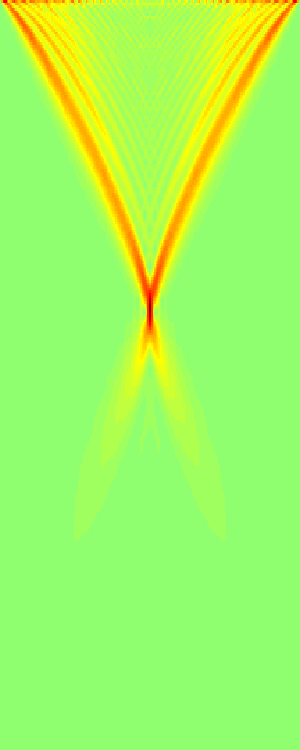
\includegraphics[height=0.5\textwidth]{assets/shear/data/F158.png}};

					% draw the borders
					\draw (0, 0) rectangle(10, 10);

					% the lesion
					\draw (6.25, 6) circle(0.5);

					% the lesion text
					\draw[<-] (6.6036, 5.6464) -- (7.25, 5);
					\draw (7.05, 5) node[right]{\scriptsize Lesion};

					% the focal point
					\draw[<-] (5, 6) -- (4, 6);
					\draw (4, 6) node[left]{\scriptsize Focal point};

					% the force distribution
					\draw[<-] (5.8, 7.75) -- (7, 7.75);
					\draw (6.8, 7.75) node[right]{\scriptsize Radiation force};

					% the focal line
					\draw[dashed] (5, 6) -- (10, 6);
					\draw[<-] (7.5, 6) -- (7.5, 6.5);
					\draw (7.5, 6.5) node[above]{\scriptsize Focal line};
				\end{tikzpicture}
				\caption[Sample radiation force distribution in relation to lesion location]{A sample acoustic radiation force distribution shown with a schematic of the lesion's location and size in the simulated tissue domain. Note how the focal point is adjacent to the lesion, offset in this case by \SI{1.25}{\cm}. The focal line extends laterally from the focal point, through the lesion, to the edge of the tissue domain---this is the line that will be used to calculate shear wave speeds.}
				\label{fig:arfi_force_shear_lesion_schematic}
			\end{figure}

		\subsection{Sample Shear Wave Speed Measurement}
		\label{subsubsec:shear_results_sample_wave_speed}
			Although measuring the shear wave speed of tissue may quantify the tissue stiffness through equation \ref{equ:shear_wave_speed_complex}, the results presented here represent the measured stiffness ratio of lesions in order to present continuity with Chapters \ref{chap:quasi-static} and \ref{chap:arfi}. In all cases where relative lesion stiffness is presented, it was calculated through comparison of the mean shear wave speed in the defined lesion region with the mean shear wave speed outside of the lesion region along the path of the lateral shear wave radiation direction. Specific ratios may be calculated using equation \ref{equ:shear_stiffness_ratio} where $E_{rel}$ is the relative stiffness ratio, $\mu_l$ and $\mu_t$ are Lam\'{e}'s second parameter for the lesion and tissue respectively, $c_{T,l}$ and $c_{T,t}$ are the shear wave speeds in the lesion and tissue respectively, and $\rho$ is the density of the tissue and assumed to be constant between the lesion and tissue.

			\begin{subequations}
				\label{equ:shear_stiffness_ratio}
				\begin{align}
					c_T &= \sqrt{\frac{\mu}{\rho}} \\
					c_T^2\rho &= \mu \\
					E_{rel} = \frac{\mu_l}{\mu_t} &= \left(\frac{c_{T,l}}{c_{T,t}}\right)^2
				\end{align}
			\end{subequations}

			In order to determine the velocity of generated shear waves, the ARFI load-induced displacement of the soft tissue must be tracked through time along a line passing through the focal point radiating laterally outward in the finite-element model of tissue deformation. A sample result of tissue displacement through time and along such a line is presented in Fig. \ref{fig:lateral_wave_i158} where the wave can be readily visualized through time, noting that the wave travels ever further from the centerline.

			\begin{figure}[!htb]
				\centering
				\begin{tikzpicture}
					\begin{axis}[
						scale only axis,
						height=2.5in,
						width=\textwidth-\widthof{100}-1in,
						xlabel={Distance from centerline, $x$ (\si{\cm})},
						ylabel={Axial displacement, $v$ (\si{\um})},
						grid=major,
						legend entries={$t = \SI{2.5}{\ms}$, $t = \SI{7.5}{\ms}$, $t = \SI{12.5}{\ms}$, $t = \SI{17.5}{\ms}$, $t = \SI{22.5}{\ms}$, $t = \SI{27.5}{\ms}$},
						legend style={legend pos=south east,font=\small},
						clip=true,
						cycle list name=SmoothColourPlotCycle,
						draw=black, text=black, fill=black,
						xmin=0, xmax=5]
						\addplot table[x expr=\thisrow{x}*100, y expr=\thisrow{v}*1e6] {assets/shear/data/shear_lateral_i158_t025.dat};
						\addplot table[x expr=\thisrow{x}*100, y expr=\thisrow{v}*1e6] {assets/shear/data/shear_lateral_i158_t075.dat};
						\addplot table[x expr=\thisrow{x}*100, y expr=\thisrow{v}*1e6] {assets/shear/data/shear_lateral_i158_t125.dat};
						\addplot table[x expr=\thisrow{x}*100, y expr=\thisrow{v}*1e6] {assets/shear/data/shear_lateral_i158_t175.dat};
						\addplot table[x expr=\thisrow{x}*100, y expr=\thisrow{v}*1e6] {assets/shear/data/shear_lateral_i158_t225.dat};
						\addplot table[x expr=\thisrow{x}*100, y expr=\thisrow{v}*1e6] {assets/shear/data/shear_lateral_i158_t275.dat};
					\end{axis}
				\end{tikzpicture}
				\caption[Sample shear wave motion through time]{Axial displacement induced by a shear wave traveling laterally across the focal line of an ARFI load. There is a stiff ($E_{rel} = 3.2$) lesion with a diameter of \SI{1}{\cm} located \SI{1.25}{\cm} away from the centerline, with both the focal line and the lesion located at a depth of \SI{4}{\cm} from the surface.}
				\label{fig:lateral_wave_i158}
			\end{figure}

			The results in Fig. \ref{fig:lateral_wave_i158} represent a finite subsample of the shear wave's propagation along the focal line. For a continuous representation of the shear wave propagation, the surface shown in Fig \ref{fig:lateral_cut_i158} may be constructed. In order to track the wave through both position and time, a contour line representing a constant displacement value may be extracted. For this work, a contour line representing the mean value of the displacement over the entire position-time domain was utilized and is portrayed in Fig. \ref{fig:lateral_cut_i158_imgsc_isoline}.

			\begin{figure}[!htb]
				\centering
				\begin{tikzpicture}
					\begin{axis}[
						scale only axis,
						enlargelimits=false,
						height=2.5in,
						width=\textwidth-\widthof{100}-1in,
						xlabel={Time, $t$ (\si{\ms})},
						ylabel={Distance from centerline, $x$ (\si{\cm})},
						axis on top,
						colormap name={RdBu},
						colorbar, point meta min=-6.6746e-01, point meta max=3.8648e-01, colorbar style={at={(1.05,0)}, anchor=south west, width=0.03\textwidth, ylabel={Axial Displacement, $v$ (\si{\um})},
							draw=black, text=black, fill=black}]
							\addplot graphics[xmin=0,xmax=31.7,ymin=0,ymax=5]{assets/shear/data/lateralCut158.png};
					\end{axis}
				\end{tikzpicture}
				\caption[Sample continuous surface plot of shear wave induced displacement]{Continous surface plot of the shear wave induced axial displacement tracked through both time and distance from the transducer centerline. The sharp transition from negative to positive displacement marks the location of shear wave in time at any given location.}
				\label{fig:lateral_cut_i158}
			\end{figure}

			\begin{figure}[!htb]
				\centering
				\begin{tikzpicture}
					\begin{axis}[
						scale only axis,
						enlargelimits=false,
						height=2.5in,
						width=\textwidth-\widthof{100}-1in,
						xlabel={Time, $t$ (\si{\ms})},
						ylabel={Distance from centerline, $x$ (\si{\cm})},
						axis on top,
						colormap name={RdBu},
						colorbar, point meta min=-6.6746e-01, point meta max=3.8648e-01, colorbar style={at={(1.05,0)}, anchor=south west, width=0.03\textwidth, ylabel={Axial Displacement, $v$ (\si{\um})}, draw=black, text=black, fill=black}]
							\addplot graphics[xmin=0,xmax=31.7,ymin=0,ymax=5]{assets/shear/data/lateralCut158.png};
							\addplot[draw=black, solid, ultra thick] table[x expr=\thisrow{t}*1000, y expr=\thisrow{x}*100] {assets/shear/data/shear_lateral_i158_isoline.dat};
							\draw[ultra thick, <->, draw=black] (axis cs:15,0.75) -- (axis cs:15,1.75);
							\draw[ultra thick, draw=black, dashed] (axis cs:0,0.75) -- (axis cs:17.5,0.75);
							\draw[ultra thick, draw=black, dashed] (axis cs:0,1.75) -- (axis cs:17.5,1.75);
							\node[right] at (axis cs:15,1.25) {Lesion};
							\draw[ultra thick, ->, draw=black] (axis cs:25.65,2.75) -- (axis cs:25.65,3.7755102040816);
							\node[below] at (axis cs:25.65,2.75) {Iso-line};
					\end{axis}
				\end{tikzpicture}
				\caption[Sample continuous surface plot of shear wave induced axial displacement highlighting the shear wave location in time]{Continuous surface plot of shear wave induced axial displacement highlighting a mean contour line representing the shear wave location as time progresses. By inspection, the slope of the contour line is greater within the lesionous region than outside of it, suggesting that the lesion is stiffer than the surrounding tissue.}
				\label{fig:lateral_cut_i158_imgsc_isoline}
			\end{figure}

			Fig. \ref{fig:lateral_cut_i158_isoline} represents the extracted contour line. This contour line now represents a position-time trace of the shear wave, from which the velocity of the wave may be calculated by differentiating the position of the wave with respect to time as per equation \ref{equ:shear_speed_differentiation}. Care must be taken when numerically differentiating, as numerical errors are greatly amplified by differentiation. To combat this, a moving window average filter with a kernel of \SI{5}{\mm} was applied to the position-time curve before center-difference differentiation was used to result in the shear wave speed graph given in Fig. \ref{fig:lateral_cut_i158_shear_wave_speed}.

			\begin{equation}
				\label{equ:shear_speed_differentiation}
				c_T = \frac{dx}{dt}
			\end{equation}

			\begin{figure}[!htb]
				\centering
				\begin{tikzpicture}
					\begin{axis}[
						scale only axis,
						height=2.5in,
						width=\textwidth-\widthof{100}-1in,
						xlabel={Time, $t$ (\si{\ms})},
						ylabel={Distance from centerline, $x$ (\si{\cm})},
						grid=major,
						clip=true,
						cycle list name=SmoothColourPlotCycle,
						draw=black, text=black, fill=black]
						\addplot table[x expr=\thisrow{t}*1000, y expr=\thisrow{x}*100] {assets/shear/data/shear_lateral_i158_isoline.dat};
					\end{axis}
				\end{tikzpicture}
				\caption[Sample extracted shear wave position-time trace]{The extracted shear wave position-time trace showing the location of the generated shear wave increases with time, albeit at different rates depending on the underlying tissue properties.}
				\label{fig:lateral_cut_i158_isoline}
			\end{figure}

			\begin{figure}[!htb]
				\centering
				\begin{tikzpicture}
					\begin{axis}[
						scale only axis,
						height=2.5in,
						width=\textwidth-\widthof{100}-1in,
						xlabel={Distance from centerline, $x$ (\si{\cm})},
						ylabel={Measured Shear Wave Speed, $c_t$ (\si{\m\per\s})},
						grid=major,
						clip=true,
						cycle list name=SmoothColourPlotCycle,
						draw=black, text=black, fill=black]
						\addplot table[x expr=\thisrow{x}*100] {assets/shear/data/shear_lateral_i158_shear_wave_speed.dat};

						\draw[ultra thick, ->, draw=black] (axis cs:0.25,2) -- (axis cs:0.75,2);
						\draw[ultra thick, <-, draw=black] (axis cs:1.75,2) -- (axis cs:2.25,2);
						\node[right] at (axis cs:2.25,2) {Lesion};
						\draw[ultra thick, draw=black, dashed] (axis cs:0.75,0) -- (axis cs:0.75,2.05);
						\draw[ultra thick, draw=black, dashed] (axis cs:1.75,0) -- (axis cs:1.75,2.05);
					\end{axis}
				\end{tikzpicture}
				\caption[Sample trace of shear wave speed through the focal line]{Trace of the shear wave speed along the focal line through both lesionous and ``healthy'' tissue. The shear wave speed within the lesion is much greater than the shear wave speed through the ``healthy'' tissue, indicating that the lesion is significantly stiffer than the surrounding tissue. The shear wave speed was calculated as the numerical differentiation of the shear wave's position through time.}
				\label{fig:lateral_cut_i158_shear_wave_speed}
			\end{figure}

			As is shown in Fig. \ref{fig:lateral_cut_i158_shear_wave_speed}, the speed of the shear wave within the lesion (which was in this case 3.2 times as stiff as the surrounding tissue) is substantially greater than the shear wave speed in the regular tissue. Note that instead of an impulse response at the boundaries of the lesion as might be expected, the shear wave speed reaches a peak value approximately halfway through the lesion, indicating that the wave requires some finite amount of time to both speed up and slow down within the lesion, suggesting that the technique may have difficulty identifying small lesions as the shear wave speed will not be able to fully adjust to the lesion in the time it takes for the wave to completely pass through the lesion.

		\FloatBarrier
		\subsection{Lesion Detection Characterization}
			In order to determine the detection sensitivity of shear wave speed quantification with respect to lesion size, hard-boundaried spherical lesions with varying radii were interrogated using ARFI loads while the speed of the shear waves developed along the focal line were monitored. The ARFI loads were applied using a probing frequency of \SI{2}{\MHz} for \SI{150}{\us} with a source pressure of \SI{3.35}{\MPa} using an F-number of $f/1.0$. The lesions were located at a depth of \SI{4}{\cm} with an offset of \SI{1.25}{\cm} from the focal point of the ARFI load. The results of this characterization are given in Fig. \ref{fig:erel_radius}. Lesions stiffness ratios were measured by calculating the maximum or minimum shear wave speed within the lesion if the shear wave speed within the lesion was greater than or less than the surrounding tissue respectively and the mean shear wave speed without the lesion and applying equation \ref{equ:shear_wave_speed}.

			\begin{figure}[!htb]
				\centering
				\begin{tikzpicture}
					\begin{axis}[
						scale only axis,
						height=2.5in,
						width=\textwidth-\widthof{100}-1in,
						xlabel={True Stiffness Ratio, $E_{rel,true}$},
						ylabel={Measured Stiffness Ratio, $E_{rel,measured}$},
						grid=major,
						legend entries={$r_{lesion} = \SI{2.5}{\mm}$, $r_{lesion} = \SI{5.0}{\mm}$, $r_{lesion} = \SI{10.0}{\mm}$, $r_{lesion} = \SI{12.5}{\mm}$},
						legend style={legend pos=north west,font=\small},
						clip=true,
						cycle list name=ColourPlotCycle,
						draw=black, text=black, fill=black]
						\addplot table {assets/shear/data/shear_radius_r025.dat};
						\addplot table {assets/shear/data/shear_radius_r050.dat};
						\addplot table {assets/shear/data/shear_radius_r100.dat};
						\addplot table {assets/shear/data/shear_radius_r125.dat};
					\end{axis}
				\end{tikzpicture}
				\caption[Numerical characterization of shear wave speed measured stiffness ratio with changing lesion radius]{Numerical characterization of the shear wave speed measured stiffness ratios acquired with varying lesion radii for a hard-boundaried lesion at a depth of \SI{4}{\cm} using an ARFI interrogation frequency of \SI{2}{\MHz}.}
				\label{fig:erel_radius}
			\end{figure}

			As can be seen in Fig. \ref{fig:erel_radius}, small lesions with radii $\leq \SI{5.0}{\mm}$ are nearly impossible to detect---large changes in the true lesion stiffness ratio represent very minute changes in the measured lesion stiffness ratio for these small lesions. Conversely, large lesions are much easier to detect, portraying a nearly one-to-one or better mapping between the true and measured lesion stiffness ratios. This suggests that the large the lesion is, the more readily it may be detected while smaller lesions are more difficult to detect with a lower limit of the lesion radius approaching \SI{5.0}{\mm}.

			\begin{figure}[!htb]
				\centering
				\begin{tikzpicture}
					\begin{axis}[
						scale only axis,
						height=2.5in,
						width=\textwidth-\widthof{100}-1in,
						major x tick style = transparent,
						ybar=2*\pgflinewidth,
						bar width=28pt,
						ymajorgrids=true,
						xlabel={Lesion Radius, $r$ (\si{\mm})},
						ylabel={Mean Squared Error},
						enlarge x limits=0.25,
						ymin=0,
						xtick=data,
						cycle list name=BarColourPlotCycle]
						\addplot table[x expr=\thisrow{radius}*1000] {assets/shear/data/shear_radius_mse.dat};
					\end{axis}
				\end{tikzpicture}
				\caption[Shear-wave speed quantified squared error related to lesion radius]{Mean squared error between the true and measured lesion stiffness ratios for increasing lesion radii for a hard-boundaried lesion at a depth of \SI{4}{\cm} using an ARFI interrogation frequency of \SI{2}{\MHz}.}
				\label{fig:erel_radius_mse}
			\end{figure}

			To further investigate these results, the mean-squared error associated with varying lesion size was calculated as per equation \ref{equ:mean-squared-error} with the results presented in Fig. \ref{fig:erel_radius_mse}. In Fig. \ref{fig:erel_radius_mse}, it is clear to see that the error associated with small lesions is significantly greater than with larger lesions. Interestingly, the largest lesions tested (with radii of \SI{12.5}{\mm}) presented greater error than lesions with radii of \SI{10.0}{\mm}. This increase in error may be largely attributed to the over-estimation of the lesion stiffness ratio for a stiff (3.2 $\times$ basal stiffness) lesion with a radius of \SI{12.5}{\mm} seen in Fig. \ref{fig:erel_radius}. The exact cause of this error is unknown. \note[KH]{Elaborate?}.

			One of the key parameters used in shear wave speed quantification is the distance between the focal point of the acoustic radiation force and the lesion itself. In order to adequately generate fully-formed shear waves within the lesion, the focal point of acoustic radiation force should be located adjacent to the lesion. As can be seen in Fig. \ref{fig:erel_doff_d4}, regardless of the lesion offset distance, shear wave speed quantification is able to differentiate lesions from the tissue with reasonable accuracy. The largest exception to this generalization is for very stiff lesions for which the ARFI load is focused the farthest away from the lesion. It is hypothesized that the measured stiffness ratio of these lesions is underestimated because by the time the shear wave reaches the relatively far-away lesion, it's energy has substantially dissipated, disallowing the wave to remain fully cohesive and speed up appropriately.

			\begin{figure}[!htb]
				\centering
				\begin{tikzpicture}
					\begin{axis}[
						scale only axis,
						height=2.5in,
						width=\textwidth-\widthof{100}-1in,
						xlabel={True Stiffness Ratio, $E_{rel,true}$},
						ylabel={Measured Stiffness Ratio, $E_{rel,measured}$},
						grid=major,
						legend entries={$\Delta_{off} = \SI{0.00}{\cm}$, $\Delta_{off} = \SI{1.25}{\cm}$, $\Delta_{off} = \SI{2.50}{\cm}$, $\Delta_{off} = \SI{3.75}{\cm}$},
						legend style={legend pos=south east,font=\small},
						clip=true,
						cycle list name=ColourPlotCycle,
						draw=black, text=black, fill=black]
						\addplot table {assets/shear/data/shear_doff_d4_o000.dat};
						\addplot table {assets/shear/data/shear_doff_d4_o125.dat};
						\addplot table {assets/shear/data/shear_doff_d4_o250.dat};
						\addplot table {assets/shear/data/shear_doff_d4_o375.dat};
					\end{axis}
				\end{tikzpicture}
				\caption[Numerical characterization of shear wave speed measured stiffness ratio with changing lesion offsets]{Numerical characterization of the shear wave speed measured stiffness ratios acquired with varying lesion offsets for a hard-boundaried \SI{0.5}{cm} radius lesion at a depth of \SI{4}{\cm} using an ARFI interrogation frequency of \SI{2}{\MHz}. The greatest error between the true and measured stiffness ratios occurred at the highest stiffness ratio of $3.2$, with the large lesion offset underestimating the stiffness ratio and the negated lesion offset overestimating the stiffness ratio.}
				\label{fig:erel_doff_d4}
			\end{figure}

			Fig. \ref{fig:erel_doff_mse_d4} portrays the mean squared error between the measured and true lesion stiffness ratios with increasing lesion offset distance. As Fig. \ref{fig:erel_doff_mse_d4} shows, a lesion offset of approximately \SI{2.5}{\cm} is ideal for quantifying lesion stiffness as it produces the least amount of error between the true and measured lesion stiffness ratios which confirms the notion that the shear wave needs some time to become fully developed as it travels through the tissue. Since the error between lesion offsets of \SI{1.25}{\cm} and \SI{2.50}{\cm} is nearly negligible, it is likely that the wave is able to become fully developed even earlier than \SI{2.50}{\cm} and lesion offsets as small as \SI{1.25}{\cm} may be used. The relatively large error present for the largest lesion offset of \SI{3.75}{\cm} is largely due to the severe underestimation of the lesion stiffness for the stiffest lesion seen in Fig. \ref{fig:erel_doff_d4}.

			\begin{figure}[!htb]
				\centering
				\begin{tikzpicture}
					\begin{axis}[
						scale only axis,
						height=2.5in,
						width=\textwidth-\widthof{100}-1in,
						major x tick style = transparent,
						ybar=2*\pgflinewidth,
						bar width=28pt,
						ymajorgrids=true,
						xlabel={Lesion Offset, $d_{off}$ (\si{\cm})},
						ylabel={Mean Squared Error},
						enlarge x limits=0.25,
						ymin=0,
						xtick=data,
						cycle list name=BarColourPlotCycle]
						\addplot table[x expr=\thisrow{doff}*100] {assets/shear/data/shear_doff_mse_d4.dat};
					\end{axis}
				\end{tikzpicture}
				\caption[Shear-wave speed quantified mean squared error related to lesion offset]{Mean squared error between the true and measured lesion stiffness ratios for increasing lesion offsets for a hard-boundaried \SI{0.5}{cm} radius lesion at a depth of \SI{4}{\cm} using an ARFI interrogation frequency of \SI{2}{\MHz}.}
				\label{fig:erel_doff_mse_d4}
			\end{figure}

			Another key parameter relating to the detection of deep tissue injury lesions relates to the depth that the lesions may actually be detected---for example, in people with large amounts of body fat or muscle, the distance between the surface of the skin and the boney prominence where lesions are most likely to form may be very large compared to someone with very little amounts of body fat or muscle. In order to study the effect of lesion depth on the detection sensitivity of shear wave speed quantification, simulated lesions were placed at various depths ranging from \SI{2}{\cm} -- \SI{8}{\cm} below the surface of the skin with the measured stiffness ratios for these lesions calculated and shown in Fig. \ref{fig:erel_depth_o250}.

			\begin{figure}[!htb]
				\centering
				\begin{tikzpicture}
					\begin{axis}[
						scale only axis,
						height=2.5in,
						width=\textwidth-\widthof{100}-1in,
						xlabel={True Stiffness Ratio, $E_{rel,true}$},
						ylabel={Measured Stiffness Ratio, $E_{rel,measured}$},
						grid=major,
						legend entries={$d = \SI{2}{\cm}$, $d = \SI{4}{\cm}$, $d = \SI{6}{\cm}$, $d = \SI{8}{\cm}$},
						legend style={legend pos=south east,font=\small},
						clip=true,
						cycle list name=ColourPlotCycle,
						draw=black, text=black, fill=black]
						\addplot table {assets/shear/data/shear_depth_o250_d2.dat};
						\addplot table {assets/shear/data/shear_depth_o250_d4.dat};
						\addplot table {assets/shear/data/shear_depth_o250_d6.dat};
						\addplot table {assets/shear/data/shear_depth_o250_d8.dat};
					\end{axis}
				\end{tikzpicture}
				\caption[Numerical characterization of shear wave speed measured stiffness ratio with changing lesion depth]{Numerical characterization of the shear wave speed measured stiffness ratios acquired with varying lesion and focal point depths for a hard-boundaried \SI{0.5}{cm} radius lesion with an offset of \SI{2.50}{\cm} using an ARFI interrogation frequency of \SI{2}{\MHz}.}
				\label{fig:erel_depth_o250}
			\end{figure}

			As Fig. \ref{fig:erel_depth_o250} shows, there is little dependence of shear wave speed quantifications detection sensitivity for shallow to medium-depth lesions---lesions placed at a depth of \SI{2}{\cm} -- \SI{6}{\cm} presented approximately equal detection curves. Of note in Fig. \ref{fig:erel_depth_o250} is that deep lesions---lesions at a depth of \SI{8}{\cm} or more---are difficult to detect as the method is not very sensitive these deeper lesions---both underestimating the stiffness of deep stiff lesions and overestimating the stiffness of deep soft lesions. The large error involved with attempting to measure the stiffness of deep lesions can be seen in Fig. \ref{fig:erel_depth_mse_o250} where the mean squared error for the various depths examined was calculated. In Fig. \ref{fig:erel_depth_mse_o250}, the \SI{8}{\cm} deep lesions present a significantly greater amount of error than their shallower counterparts. Also of note is that the shallowest lesions investigated---lesions at a depth of \SI{2}{\cm}---presented with greater error than the mid-depth lesions. The source of this error largely lies in the overestimation of the stiff lesion stiffness seen in Fig. \ref{fig:erel_depth_o250} which may be due to numerical errors in the models and calculations.

			\begin{figure}[!htb]
				\centering
				\begin{tikzpicture}
					\begin{axis}[
						scale only axis,
						height=2.5in,
						width=\textwidth-\widthof{100}-1in,
						major x tick style = transparent,
						ybar=2*\pgflinewidth,
						bar width=28pt,
						ymajorgrids=true,
						xlabel={Lesion Depth, $d$ (\si{\cm})},
						ylabel={Mean Squared Error},
						enlarge x limits=0.25,
						ymin=0,
						xtick=data,
						cycle list name=BarColourPlotCycle]
						\addplot table[x expr=\thisrow{depth}*100] {assets/shear/data/shear_depth_mse_o250.dat};
					\end{axis}
				\end{tikzpicture}
				\caption[Shear-wave speed quantified mean squared error related to lesion depth]{Mean squared error between the true and measured lesion stiffness ratios for increasing lesion depths for a hard-boundaried \SI{0.5}{cm} radius lesion with an offset of \SI{2.50}{\cm} using an ARFI interrogation frequency of \SI{2}{\MHz}.}
				\label{fig:erel_depth_mse_o250}
			\end{figure}

			Since deep tissue injury lesions are unlikely to be perfectly round and hard-boundaried, three different models of lesion geometry were investigated---namely, lesions with blurred boundaries that ``fade'' into the surrounding tissue, clusters of small lesions that together make up a larger lesions region, and a lesion with mri-acquired geometry \cite{solis13} embedded in geometry obtained from a Visible Human slice \cite{visiblehuman}. Although the spherical hard-boundaried lesions may not represent all the intricacies of real deep tissue injuries, the general trends that result from analysing them may improve the general understanding of lesion detection behaviour.

			In order to investigate the effect of blurring lesions into the background tissue, hard-boundaried spherical lesions were blurred with varying blur radii as described in Section \ref{subsec:model_setup}. The results of this characterization are presented in Fig. \ref{fig:erel_blur}. As can be seen in Fig. \ref{fig:erel_blur}, the effect of blur radii on lesion detection ability is negligible as noted by how the detection curves of the lesions with varying blur radii are largely coincident.

			\begin{figure}[!htb]
				\centering
				\begin{tikzpicture}
					\begin{axis}[
						scale only axis,
						height=2.5in,
						width=\textwidth-\widthof{100}-1in,
						xlabel={True Stiffness Ratio, $E_{rel,true}$},
						ylabel={Measured Stiffness Ratio, $E_{rel,measured}$},
						grid=major,
						legend entries={$b_r = \SI{2.5}{\mm}$, $b_r = \SI{5.0}{\mm}$, $b_r = \SI{7.5}{\mm}$},
						legend style={legend pos=south east,font=\small},
						clip=true,
						cycle list name=ColourPlotCycle,
						draw=black, text=black, fill=black]
						\addplot table {assets/shear/data/shear_blur_r25.dat};
						\addplot table {assets/shear/data/shear_blur_r50.dat};
						\addplot table {assets/shear/data/shear_blur_r75.dat};
					\end{axis}
				\end{tikzpicture}
				\caption[Numerical characterization of shear wave speed measured stiffness ratio with blurred lesions]{Numerical characterization of the shear wave speed measured stiffness ratios acquired with varying lesion and focal point depths for a blurred \SI{1.0}{cm} radius lesion with an offset of \SI{1.25}{\cm} at a depth of \SI{4}{\cm} using an ARFI interrogation frequency of \SI{2}{\MHz}.}
				\label{fig:erel_blur}
			\end{figure}

			This lack of reliance of detection sensitivity on blur radius is further portrayed by the mean squared error of the results, calculated in Fig. \ref{fig:erel_blur_mse}. While there are some minor differences in the error between the various blur radii---chiefly between blur radii of \SI{2.5}{\mm} and \SI{5.0}{\mm}---the scale of these differences lie within the range of numerical error and noise and so is not significant.

			The fact that detection sensitivity does not decrease with increasing blur radii in shear wave speed quantification makes shear wave speed quantification a desirable tool for detecting deep tissue injury lesions as it means that even imperfect, newly-forming lesions can still be readily detected and monitored.

			\begin{figure}[!htb]
				\centering
				\begin{tikzpicture}
					\begin{axis}[
						scale only axis,
						height=2.5in,
						width=\textwidth-\widthof{100}-1in,
						major x tick style = transparent,
						ybar=2*\pgflinewidth,
						bar width=28pt,
						ymajorgrids=true,
						xlabel={Lesion Blur Radius, $b_r$ (\si{\mm})},
						ylabel={Mean Squared Error},
						enlarge x limits=0.25,
						ymin=0,
						xtick=data,
						cycle list name=BarColourPlotCycle]
						\addplot table[x expr=\thisrow{blur}*1000] {assets/shear/data/shear_blur_mse.dat};
					\end{axis}
				\end{tikzpicture}
				\caption[Shear-wave speed quantified mean squared error related to lesion blurring]{Mean squared error between the true and measured lesion stiffness ratios for increasing lesion depths for a blurred \SI{1.0}{cm} radius lesion with an offset of \SI{1.25}{\cm} at a depth of \SI{4}{\cm} using an ARFI interrogation frequency of \SI{2}{\MHz}.}
				\label{fig:erel_blur_mse}
			\end{figure}

			Beyond having boundaries that ``fade'' into the background tissue, deep tissue injury lesions may in fact be heterogeneous in nature with a large number of small lesions clustered together to form a larger lesionous region. To investigate this phenomenon, the effect of small clustered lesion density and individual radii were investigated using shear wave speed quantification. The effect of clustered lesion density was investigated as outlined in Section \ref{subsec:model_setup}, the results of which are shown in Fig. \ref{fig:erel_cluster_density}. \note[KH]{Add graph of shear wave speed along focal line for clustered lesions to show lack of ability to detect individual small lesions?}

			As Fig. \ref{fig:erel_cluster_density} shows, decreasing the cluster density generally results in a decreasing detection sensitivity with the least dense clusters both underestimating the stiffness of stiff lesions and overestimating the stiffness of soft lesions. This behaviour is somewhat expected---as the density of clustered lesions decreases, so too does the mean true stiffness of the lesionous region that is inspected due to the greater ratio of ``healthy'' tissue to lesionous tissue.

			\begin{figure}[!htb]
				\centering
				\begin{tikzpicture}
					\begin{axis}[
						scale only axis,
						height=2.5in,
						width=\textwidth-\widthof{100}-1in,
						xlabel={True Stiffness Ratio, $E_{rel,true}$},
						ylabel={Measured Stiffness Ratio, $E_{rel,measured}$},
						grid=major,
						legend entries={$b_\rho = \SI{10}{\per\cm\squared}$, $b_\rho = \SI{20}{\per\cm\squared}$, $b_\rho = \SI{30}{\per\cm\squared}$, $b_\rho = \SI{40}{\per\cm\squared}$},
						legend style={legend pos=south east,font=\small},
						clip=true,
						cycle list name=ColourPlotCycle,
						draw=black, text=black, fill=black]
						\addplot table {assets/shear/data/shear_cluster_dens_d10.dat};
						\addplot table {assets/shear/data/shear_cluster_dens_d20.dat};
						\addplot table {assets/shear/data/shear_cluster_dens_d30.dat};
						\addplot table {assets/shear/data/shear_cluster_dens_d40.dat};
					\end{axis}
				\end{tikzpicture}
				\caption[Numerical characterization of shear wave speed measured stiffness ratio with clustered lesions]{Numerical characterization of the shear wave speed measured stiffness ratios acquired with varying cluster densities for clustered \SI{1}{\mm} radius lesions within a \SI{1.0}{cm} radius with an offset of \SI{1.25}{\cm} at a depth of \SI{4}{\cm} using an ARFI interrogation frequency of \SI{2}{\MHz}.}
				\label{fig:erel_cluster_density}
			\end{figure}

			This generalization is further portrayed in by the mean squared error which is shown in Fig. \ref{fig:erel_cluster_density_mse}. In Fig. \ref{fig:erel_cluster_density_mse}, increasing cluster density results in monotonically decreasing error.

			\begin{figure}[!htb]
				\centering
				\begin{tikzpicture}
					\begin{axis}[
						scale only axis,
						height=2.5in,
						width=\textwidth-\widthof{100}-1in,
						major x tick style = transparent,
						ybar=2*\pgflinewidth,
						bar width=28pt,
						ymajorgrids=true,
						xlabel={Lesion Cluster Density, $b_\rho$ (\si{\per\cm\squared})},
						ylabel={Mean Squared Error},
						enlarge x limits=0.25,
						ymin=0,
						xtick=data,
						cycle list name=BarColourPlotCycle]
						\addplot table {assets/shear/data/shear_cluster_dens_mse.dat};
					\end{axis}
				\end{tikzpicture}
				\caption[Shear-wave speed quantified mean squared error related to small lesion cluster density]{Mean squared error between the true and measured lesion stiffness ratios for increasing lesion cluster density for clustered \SI{1}{\mm} radius lesions within a \SI{1.0}{cm} radius with an offset of \SI{1.25}{\cm} at a depth of \SI{4}{\cm} using an ARFI interrogation frequency of \SI{2}{\MHz}.}
				\label{fig:erel_cluster_density_mse}
			\end{figure}

			Beyond the cluster density, the size of individual clustered lesions within the lesionous region may affect the detection sensitivity. To investigate this parameter, the radii of the individual lesions in the clustered lesion model were varied, with the results presented in Fig. \ref{fig:erel_cluster_radius}. Fig. \ref{fig:erel_cluster_radius} shows how decreasing the individual clustered lesion radii results in decreases in the detection sensitivity. This is similar to the results presented in Fig. \ref{fig:erel_cluster_density} in that decreasing the individual lesion radii results in a decrease of the ratio between lesionous tissue and healthy tissue within the lesionous region---the greater the proportion of lesionous tissue within the investigated region, the more accurate the detection of the lesionous region.

			\begin{figure}[!htb]
				\centering
				\begin{tikzpicture}
					\begin{axis}[
						scale only axis,
						height=2.5in,
						width=\textwidth-\widthof{100}-1in,
						xlabel={True Stiffness Ratio, $E_{rel,true}$},
						ylabel={Measured Stiffness Ratio, $E_{rel,measured}$},
						grid=major,
						legend entries={$r_{bl} = \SI{0.5}{\mm}$, $r_{bl} = \SI{1.0}{\mm}$, $r_{bl} = \SI{1.5}{\mm}$},
						legend style={legend pos=south east,font=\small},
						clip=true,
						cycle list name=ColourPlotCycle,
						draw=black, text=black, fill=black]
						\addplot table {assets/shear/data/shear_cluster_radius_r05.dat};
						\addplot table {assets/shear/data/shear_cluster_radius_r10.dat};
						\addplot table {assets/shear/data/shear_cluster_radius_r15.dat};
					\end{axis}
				\end{tikzpicture}
				\caption[Numerical characterization of shear wave speed measured stiffness ratio with clustered lesions]{Numerical characterization of the shear wave speed measured stiffness ratios acquired with varying clustered lesion radii for clustered lesions with a density of \SI{30}{\per\cm\squared} within a \SI{1.0}{cm} radius with an offset of \SI{1.25}{\cm} at a depth of \SI{4}{\cm} using an ARFI interrogation frequency of \SI{2}{\MHz}.}
				\label{fig:erel_cluster_radius}
			\end{figure}

			Again, this conclusion is corroborated by the mean squared error shown in Fig. \ref{fig:erel_cluster_radius_mse}. In Fig. \ref{fig:erel_cluster_radius_mse}, increasing the individual lesion radii results in a significant decrease in the stiffness measurement error in the lesionous region.

			\begin{figure}[!htb]
				\centering
				\begin{tikzpicture}
					\begin{axis}[
						scale only axis,
						height=2.5in,
						width=\textwidth-\widthof{100}-1in,
						major x tick style = transparent,
						ybar=2*\pgflinewidth,
						bar width=28pt,
						ymajorgrids=true,
						xlabel={Clustered Lesion Radius, $r_{bl}$ (\si{\mm})},
						ylabel={Mean Squared Error},
						enlarge x limits=0.25,
						ymin=0,
						xtick=data,
						cycle list name=BarColourPlotCycle]
						\addplot table[x expr=\thisrow{radius}*1000] {assets/shear/data/shear_cluster_radius_mse.dat};
					\end{axis}
				\end{tikzpicture}
				\caption[Shear-wave speed quantified mean squared error related to small lesion cluster density]{Mean squared error between the true and measured lesion stiffness ratios for increasing clustered lesion radii for clustered lesions with a density of \SI{30}{\per\cm\squared} within a \SI{1.0}{cm} radius with an offset of \SI{1.25}{\cm} at a depth of \SI{4}{\cm} using an ARFI interrogation frequency of \SI{2}{\MHz}.}
				\label{fig:erel_cluster_radius_mse}
			\end{figure}

			Finally, in order to place these characterizations within the context of a real deep tissue injury situated within the geometry of a real human soft tissue domain, a numerical characterization of lesion size in the Visible Human lesion model outlined in Section \ref{subsec:model_setup} was carried out with the results portrayed in Fig. \ref{fig:erel_human_radius}. Fig. \ref{fig:erel_human_radius} relates the change in detection sensitivity with different sized lesions and shows that small lesions (with ``radii'' $\leq$ \SI{5.0}{\mm}) are extremely difficult to detect as the stiffness of small stiff lesions is severely underestimated and the stiffness of small soft lesions is severely overestimated. These results align with what was seen in the spherical hard-boundaried lesion case presented in Fig. \ref{fig:erel_radius}, indicating that the simplified spherical results generally hold true for the more complex geometry results.

			\begin{figure}[!htb]
				\centering
				\begin{tikzpicture}
					\begin{axis}[
						scale only axis,
						height=2.5in,
						width=\textwidth-\widthof{100}-1in,
						xlabel={True Stiffness Ratio, $E_{rel,true}$},
						ylabel={Measured Stiffness Ratio, $E_{rel,measured}$},
						grid=major,
						legend entries={$r_{lesion} = \SI{2.5}{\mm}$, $r_{lesion} = \SI{5.0}{\mm}$, $r_{lesion} = \SI{10.0}{\mm}$, $r_{lesion} = \SI{12.5}{\mm}$},
						legend style={legend pos=south east,font=\small},
						clip=true,
						cycle list name=ColourPlotCycle,
						draw=black, text=black, fill=black]
						\addplot table {assets/shear/data/shear_human_radius_r025.dat};
						\addplot table {assets/shear/data/shear_human_radius_r050.dat};
						\addplot table {assets/shear/data/shear_human_radius_r100.dat};
						\addplot table {assets/shear/data/shear_human_radius_r125.dat};
					\end{axis}
				\end{tikzpicture}
				\caption[Numerical characterization of shear wave speed measured stiffness ratio with changing lesion radii in a visible human model]{Numerical characterization of shear wave speed measured stiffness ratio with changing lesion radii for MRI-acquired lesion geometry in a Visible Human model with an offset of \SI{1.25}{\cm} at a depth of \SI{6}{\cm} using an ARFI interrogation frequency of \SI{2}{\MHz}.}
				\label{fig:erel_human_radius}
			\end{figure}

			As expected from the results in Fig. \ref{fig:erel_human_radius}, increasing the lesion radius results in monotonically decreasing measurement error as is shown in Fig. \ref{fig:erel_human_radius_mse} with the least amount of measurement error present for the largest lesions. This means that relatively larger lesions will be easier to detect and accurately quantify and may be due to the shear wave requiring some finite period of time to speed up or slow down with a lesionous region of tissue as discussed previously.

			\begin{figure}[!htb]
				\centering
				\begin{tikzpicture}
					\begin{axis}[
						scale only axis,
						height=2.5in,
						width=\textwidth-\widthof{100}-1in,
						major x tick style = transparent,
						ybar=2*\pgflinewidth,
						bar width=28pt,
						ymajorgrids=true,
						xlabel={Lesion Radius, $r$ (\si{\mm})},
						ylabel={Mean Squared Error},
						enlarge x limits=0.25,
						ymin=0,
						xtick=data,
						cycle list name=BarColourPlotCycle]
						\addplot table[x expr=\thisrow{radius}*1000] {assets/shear/data/shear_human_radius_mse.dat};
					\end{axis}
				\end{tikzpicture}
				\caption[Shear-wave speed quantified mean squared error related to MRI-acquired lesion size in a Visible Human model]{Mean squared error between the true and measured lesion stiffness ratios for increasing lesion radii for MRI-acquired lesion geometry in a Visible Human model with an offset of \SI{1.25}{\cm} at a depth of \SI{6}{\cm} using an ARFI interrogation frequency of \SI{2}{\MHz}.}
				\label{fig:erel_human_radius_mse}
			\end{figure}

		\FloatBarrier
		\subsection{Physical Phantom Validation}
			In order to examine the validity of the simulations presented in Section \ref{subsec:model_setup} and the results presented in Section \ref{subsec:shear_results}, experiments using a physical tissue mimicking phantom and an ultrasound machine were performed as described in Section \ref{subsec:shear_model_validation}. The results of these experiments are presented in Figs. \ref{fig:shear_phantom_validation_nominal} and \ref{fig:shear_phantom_validation} where the difference between the experimentally measured stiffness ratios of lesions were compared against their nominal and simulated stiffnesses respectively.

			\begin{figure}[!htb]
				\centering
				\begin{tikzpicture}
					\begin{axis}[
						scale only axis,
						height=3in,
						width=\textwidth-\widthof{100}-1in,
						xlabel={Nominal Stiffness Ratio, $E_{nominal}$},
						ylabel style={align=center},
						ylabel={Experimentally Measured \\ Stiffness Ratio, $E_{exp,measured}$},
						legend entries={Results, Ideal},
						legend style={legend pos=south east,font=\small},grid=major,clip=true,cycle list name=ColourPlotCycle,
						xmin=0, xmax=4,
						ymin=0, ymax=4,
						draw=black, text=black, fill=black]
							\addplot+[
								error bars/.cd,
								y dir=both,
								y explicit,
								error bar style={ultra thick},
								error mark options={
									rotate=90,
									mark size=8pt,
									ultra thick
								}] table[y error plus=upper, y error minus=lower] {assets/shear/data/shear_experiment_nominal.dat};
							\addplot[mark=none,dashed,ultra thick] plot coordinates {(0, 0) (4, 4)};
					\end{axis}
				\end{tikzpicture}
				\caption[Experimental shear wave speed quantification results]{Relation between nominally reported strain ratios of the tissue mimicking phantom and experimentally measured strain ratios for a lesion at a depth of \SI{3.5}{\cm} and diameter of \SI{2.0}{\cm} showing general agreement between simulated and experimental cases. Error bars represent the range of measurements acquired.}
				\label{fig:shear_phantom_validation_nominal}
			\end{figure}

			Fig. \ref{fig:shear_phantom_validation_nominal} shows the general agreement between the nominal and experimentally acquired lesion stiffness ratios. Of note is the increasing amount of measurement error associated with increasing nominal stiffness ratios and reflects the general underestimation of stiff lesion stiffness that was seen in the characterization of nearly all stiff lesions in Section \ref{subsec:shear_results}. Further, the relatively large degree of error was due to the measurement of the shear wave speed within the lesion rather than variability in the shear wave speed of the surrounding tissue. Nonetheless, the experimentally-acquired values lay within error of the expected nominal stiffness ratios, so the experiment was considered to produce acceptable results to compare against the simulations. The results of this comparison are shown in Fig. \ref{fig:shear_phantom_validation} where the stiffness ratios acquired through simulation are compared against experimentally-acquired stiffness ratios of parametrically identical lesions.

			\begin{figure}[!htb]
				\centering
				\begin{tikzpicture}
					\begin{axis}[
						scale only axis,
						height=3in,
						width=\textwidth-\widthof{100}-1in,
						xlabel={Experimentally Measured Stiffness Ratio, $E_{exp,measured}$},
						ylabel style={align=center},
						ylabel={Simulated Measured \\ Stiffness Ratio, $E_{sim,measured}$},
						legend entries={Results, Ideal},
						legend style={legend pos=south east,font=\small},grid=major,clip=true,cycle list name=ColourPlotCycle,
						xmin=0, xmax=4,
						ymin=0, ymax=4,
						draw=black, text=black, fill=black]
							\addplot+[
								error bars/.cd,
								x dir=both,
								x explicit,
								error bar style={ultra thick},
								error mark options={
									rotate=90,
									mark size=8pt,
									ultra thick
								}] table[x error plus=upper, x error minus=lower] {assets/shear/data/shear_experiment.dat};
							\addplot[mark=none,dashed,ultra thick] plot coordinates {(0, 0) (4, 4)};
					\end{axis}
				\end{tikzpicture}
				\caption[Experimental validation of shear wave speed quantification model results]{Relation between simulated measured strain ratios and experimental measured strain ratios for a lesion at a depth of \SI{3.5}{\cm} and diameter of \SI{2.0}{\cm} showing general agreement between simulated and experimental cases.}
				\label{fig:shear_phantom_validation}
			\end{figure}

			As expected, there is nearly a one-to-one correspondence between the experimentally measured lesion stiffness ratios and the simulated lesion stiffness ratios for the various lesions investigated. In all of the lesion cases studied, the simulated lesion stiffness ratio was slightly greater than the experimentally measured stiffness ratio. This suggests that the simulated models introduce a minor bias in the results, although as the correlation is linear this is may be readily accounted for. Another key observation is that the underestimated lesion stiffness ratio for stiff lesions that was seen in Fig. \ref{fig:shear_phantom_validation_nominal} correlates well with the results obtained experimentally.

	\section{Conclusions}
		The results given in Section \ref{subsec:shear_results} represent a numerical characterization of the use of the ultrasound elastography technique of shear wave speed quantification toward the detection and monitoring of early and progressive deep tissue injuries. This work presents arguably the most useful technology for monitoring deep tissue injury progression as it provides quantitative measures of lesion stiffnesses as opposed to the qualitative measures provided by quasi-static elastography and acoustic radiation force impulse imaging.

		The results presented here show that shear wave speed quantification is a viable tool for both detecting and monitoring deep tissue injuries, provided the injuries are in general greater than \SI{1}{\cm} in diameter and are closer to the surface of the skin than \SI{8}{\cm}. In order to provide the most accurate results, ARFI focal points should be located approximately \SI{1.25}{\cm} -- \SI{2.50}{\cm} away from the desired region of interest, allowing the shear waves to fully develop before they pass through the lesion for measurement. Blurring the lesions had no appreciable effect on the detection sensitivity whatsoever, however clusters of small lesions comprising a larger lesionous region did---reducing the area ratio of lesionous tissue to that of healthy tissue consistently resulted in lower detection sensitivities. To relate the findings from the simpler model geometries, a simulated lesion with MRI-acquired geometry was placed in a cross-sectional slice of human tissue with geometry obtained from the Visible Human project. The results of the numerical characterizations were consistent with those found using a simpler, spherical model. Finally, the entire simulation pipeline was validated using a tissue mimicking phantom and an ultrasound machine capable of performing shear wave speed quantification where physical lesions presented similar results to their simulated counterparts.

		With a firm understanding of the parameters that affect deep tissue injury detection using shear wave speed quantification, future work may entail investigating the use of shear wave speed quantification in both animal and human subjects who are either at an elevated risk of developing deep tissue injuries or are known to be suffering from such injuries. These steps will be necessary before the technique may be used in a clinical setting---an eventuality that will hopefully result from this work.